\documentclass[a4paper, 12pt]{article}
\usepackage[T1]{fontenc}
\usepackage{lmodern}
\usepackage{color}
\usepackage{amsfonts}
\usepackage{epstopdf}
\usepackage{matlab}
\usepackage{booktabs}
\usepackage{blindtext}
\usepackage{hyperref}
\usepackage[brazil]{babel}
\usepackage{amssymb}
\usepackage[utf8]{inputenc}
\usepackage{amsmath}
\usepackage{graphicx}
\usepackage{adjustbox}
\usepackage{float}
\usepackage{caption}
\usepackage{indentfirst}
\usepackage{listings}
\usepackage{tcolorbox}
\usepackage{upgreek}
\usepackage{multicol,lipsum}
\usepackage[a4paper, top=3cm, left=3cm, bottom=3cm, right=3cm]{geometry}
\usepackage{setspace}
\usepackage{pdfpages}
\usepackage{multirow}
\usepackage[dvipsnames]{xcolor}
\usepackage[table]{xcolor}
\usepackage[DIV=15]{typearea}
\usepackage[nottoc]{tocbibind}
\usepackage[sort,numbers]{natbib}
\usepackage{matlab}
\usepackage{listings}

\lstdefinestyle{python}{
  language=Python,
  basicstyle=\ttfamily,
  keywordstyle=\color{blue},
  stringstyle=\color{green},
  commentstyle=\color{gray},
  numbers=left,
  numberstyle=\tiny\color{gray},
  stepnumber=1,
  numbersep=5pt,
  backgroundcolor=\color{white},
  showspaces=false,
  showstringspaces=false,
  showtabs=false,
  frame=single,
  rulecolor=\color{black},
  tabsize=4,
  captionpos=b,
  breaklines=true,
  breakatwhitespace=false,
  title=\lstname,
  escapeinside={\%*}{*)},
  morekeywords={self},
  emph={MyClass,__init__},
  emphstyle=\color{red}
}

\begin{document}

\begin{titlepage}
    \begin{center}
        \vspace{10pt}
        \begin{figure}[!ht]
            \centering
            
\includegraphics{images/puc-rio-logo.png}
        \end{figure}
        \huge{Inteligência Computacional Aplicada}
        \vspace{70pt}
        
        \textbf{ENG1456}
        \textbf{\large{\\ }}
        
        \vspace{30pt}
        \textbf{\small{\\LÓGICA FUZZY}}

        \vspace{75pt}
        
    \end{center}
    
    \begin{flushleft}
        \begin{tabbing}
        Aluno(a)\qquad\qquad\=\>Paloma Fernanda Loureiro Sette - 1621595\\
        Professor(a)\>Ricardo Tanscheit\\
        \end{tabbing}
    \end{flushleft}
    \begin{center}
        \vspace{215pt}
        Rio de Janeiro, 27 de Junho de 2024
    \end{center}
\end{titlepage}

\newpage
\tableofcontents
\thispagestyle{empty}

\newpage
\pagenumbering{arabic}

\newpage

\listoffigures
\thispagestyle{empty}

\newpage

\section{Introdução}
Este relatório tem como objetivo descrever o desenvolvimento do primeiro trabalho de Lógica Fuzzy, que compõe a disciplina de Inteligência Computacional Aplicada. O trabalho consiste na criação de um Sistema de Inferência Fuzzy (SIF) para previsão de séries temporais, utilizando a metodologia de Wang \& Mendel para extração de regras fuzzy a partir dos dados fornecidos. Para obter o melhor desempenho possível, foram realizadas diversas alterações nos parâmetros do SIF, como o número de conjuntos fuzzy, o tamanho da janela de observação, as operações de interseção dos antecedentes, as operações de implicação e os métodos de defuzzificação.\\

Para este trabalho, foi designada a base de dados \textit{"stock\_data\_part\_10.csv"}, cujas informações consistem numa série temporal dos preços de uma determinada ação na bolsa de valores.


\newpage
\section{Parte 1: Sistema de Inferência Fuzzy (SIF)}

Deseja-se realizar uma previsão de um passo a frente, por meio de um sistema de inferência fuzzy
(SIF). Para tal, é necessário efetuar uma extração de regras a partir dos dados fornecidos utilizando
o método de Wang \& Mendel. Construiremos esse SIF utilizando Python. Em seguida, buscaremos pelo melhor desempenho possível, realizando alterações no número de
conjuntos fuzzy, no tamanho da janela e nas operações de interseção dos antecedentes,
implicação e defuzzificação.

\subsection{Construção em Python}
O objetivo principal foi realizar uma previsão de um passo à frente utilizando um Sistema de Inferência Fuzzy (SIF). A metodologia de Wang \& Mendel foi utilizada para extração de regras fuzzy a partir dos dados fornecidos. O procedimento foi dividido nas seguintes etapas:

\subsubsection{Funções Auxiliares}

A fim de otimizar os testes, foram criadas funções auxiliares para mais praticidade e organização.

\begin{itemize}
    \item \textbf{Carregamento dos dados e criação de lags}
\end{itemize}

A função \texttt{charge\_data} é responsável pelo carregamento dos dados de um arquivo CSV e pela seleção da coluna de interesse, que será renomeada para \texttt{target}. A função retorna um DataFrame contendo apenas a coluna selecionada.

\begin{figure}[H]
    \centering
    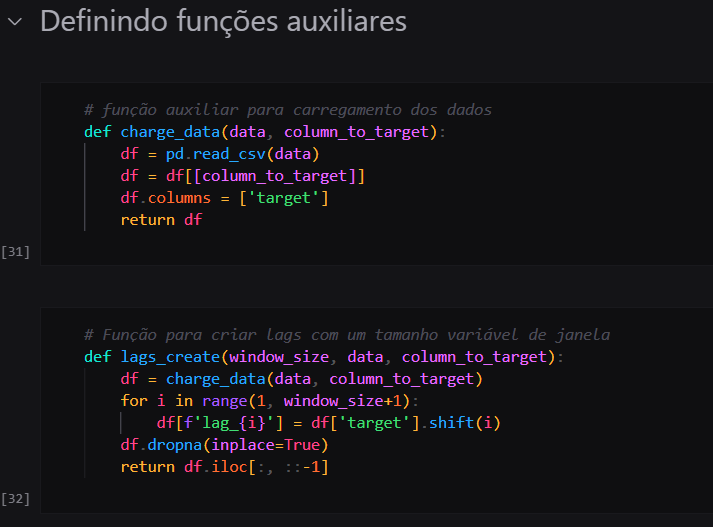
\includegraphics[scale=0.6]{images/aux_functions_1.png}
    \caption{Funções auxiliares para carregamento de dados e criação de lags.}
    \label{fig:aux_functions_1}
\end{figure}



A função \texttt{lags\_create} cria lags com um tamanho variável de janela. Primeiro, ela carrega os dados utilizando a função \texttt{charge\_data}. Em seguida, para cada tamanho de janela especificado, cria uma nova coluna no DataFrame para cada lag. O DataFrame resultante é retornado com as colunas na ordem inversa.\\


\begin{itemize}
    \item \textbf{Criação de variáveis fuzzy}
\end{itemize}
A função \texttt{create\_fuzzy\_variables} é responsável por criar variáveis fuzzy com um número variável de conjuntos fuzzy e aplicar o método de defuzzificação especificado. Ela calcula os valores mínimos e máximos do DataFrame, cria uma lista de variáveis fuzzy (antecedentes e consequentes) e define automaticamente os conjuntos fuzzy para cada variável.

\begin{figure}[H]
    \centering
    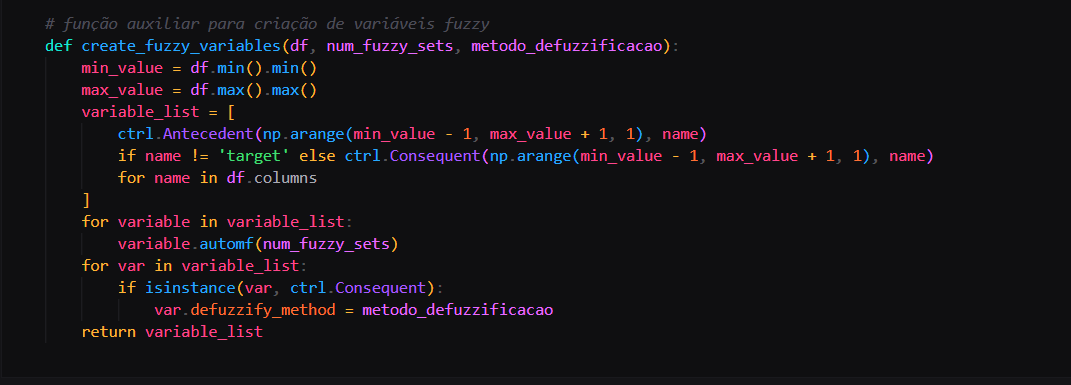
\includegraphics[scale=0.6]{images/aux_functions_2.png}
    \caption{Função auxiliar para criação de variáveis fuzzy.}
    \label{fig:aux_functions_2}
\end{figure}


\begin{itemize}
    \item \textbf{Operações de interseção}
\end{itemize}

As funções \texttt{operacao\_intersecao\_min}, \texttt{operacao\_intersecao\_prod} e \texttt{operacao\_intersecao\_avg} são responsáveis por calcular a interseção entre os antecedentes de diferentes maneiras: mínimo, produto e média, respectivamente.

\begin{figure}[H]
    \centering
    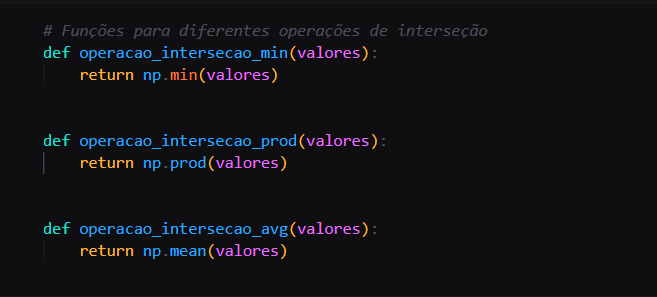
\includegraphics[scale=0.6]{images/aux_functions_3.png}
    \caption{Funções para diferentes operações de interseção.}
    \label{fig:aux_functions_3}
\end{figure}


\begin{itemize}
    \item \textbf{Implicações}
\end{itemize}

As funções \texttt{implicacao\_min}, \texttt{implicacao\_prod} e \texttt{implicacao\_maxmin} são responsáveis por calcular a implicação dos antecedentes nos consequentes de diferentes maneiras: mínimo, produto e soma truncada, respectivamente.

\begin{figure}[H]
    \centering
    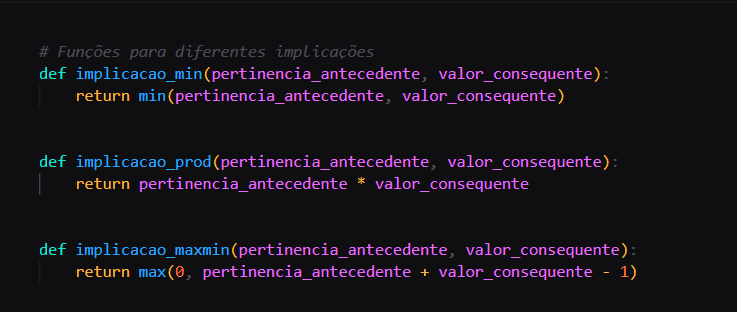
\includegraphics[scale=0.6]{images/aux_functions_4.png}
    \caption{Funções para diferentes operações de implicação.}
    \label{fig:aux_functions_4}
\end{figure}


\begin{itemize}
    \item \textbf{Métodos de defuzzificação}
\end{itemize}
As funções \texttt{defuzzificacao\_centroid}, \texttt{defuzzificacao\_mean\_of\_maxima} e \texttt{defuzzificacao\_weighted\_average} são responsáveis por realizar a defuzzificação utilizando diferentes métodos: centroide, média dos máximos e média ponderada, respectivamente.

\begin{figure}[H]
    \centering
    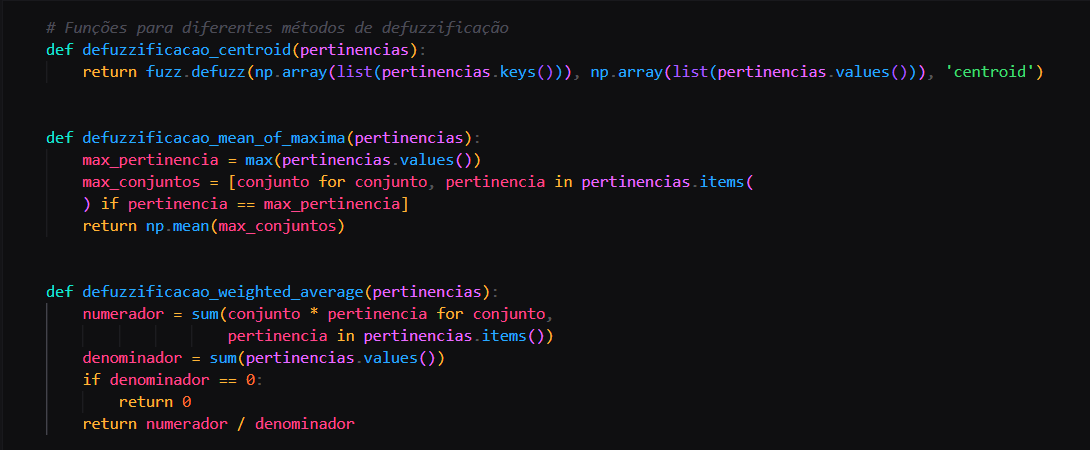
\includegraphics[scale=0.6]{images/aux_functions_5.png}
    \caption{Funções para diferentes métodos de defuzzificação.}
    \label{fig:aux_functions_5}
\end{figure}


\begin{itemize}
    \item \textbf{Predição e avaliação do modelo}
\end{itemize}
A função \texttt{predict} utiliza o sistema de inferência fuzzy para realizar a previsão dos valores de saída com base nas entradas fornecidas. A função \texttt{avaliar\_modelo} calcula o erro quadrático médio (MSE) entre os valores reais e os valores preditos, retornando o MSE e o DataFrame contendo as previsões.

\begin{figure}[H]
    \centering
    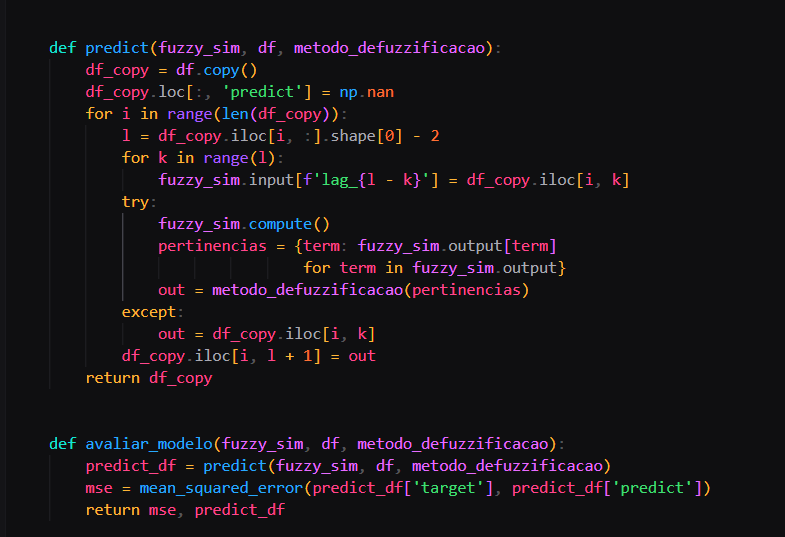
\includegraphics[scale=0.6]{images/aux_functions_6.png}
    \caption{Funções de predição e avaliação do modelo.}
    \label{fig:aux_functions_6}
\end{figure}


\subsubsection{Configuração e Otimização do Sistema}
Para otimizar o mapeamento das funções auxiliares durante os testes, foram criados dicionários que associam as funções de interseção, implicação e defuzzificação aos seus respectivos nomes:


Os dicionários criados são:

\begin{itemize}
    \item \texttt{dic\_operacoes\_intersecao}: Define os métodos de interseção que podem ser utilizados no sistema fuzzy. As opções incluem Mínimo, Produto e Média.
    \item \texttt{dic\_implicacoes}: Define os métodos de implicação. As opções incluem Mínimo, Soma Truncada e Produto.
    \item \texttt{dic\_defuzzificacao}: Define os métodos de defuzzificação. As opções incluem Centro de Gravidade, Média dos Máximos e Média Ponderada.
\end{itemize}

\begin{figure}[H]
    \centering
    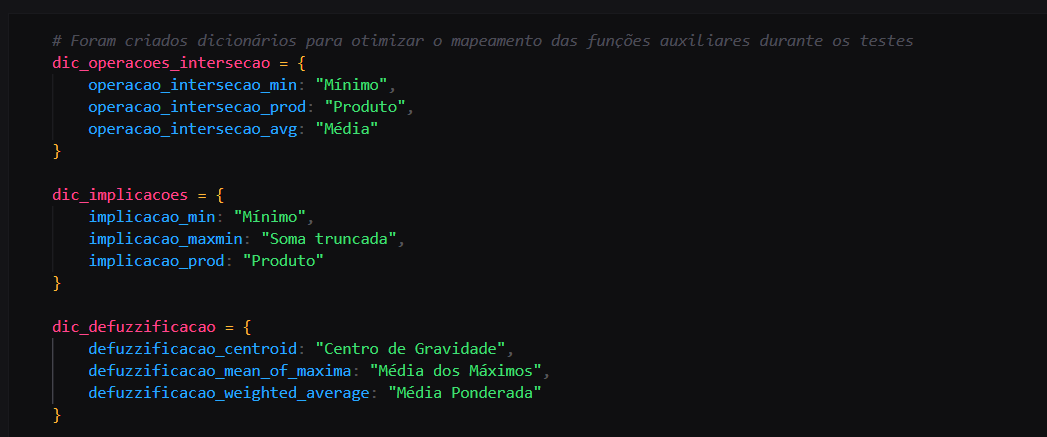
\includegraphics[scale=0.6]{images/dicionarios.png}
    \caption{Dicionários de operações para interseção, implicação e defuzzificação.}
    \label{fig:parametros_1}
\end{figure}


\textbf{Parâmetros para Busca do Melhor Desempenho}

Para encontrar a melhor configuração do sistema, os seguintes parâmetros foram definidos e alterados durante os testes:


\begin{itemize}
    \item \texttt{window\_size}: Tamanho da janela utilizada na criação dos lags. Exemplo: 7.
    \item \texttt{num\_fuzzy\_sets}: Número de conjuntos fuzzy. Exemplo: 5.
    \item \texttt{metodo\_defuzzificacao}: Método de defuzzificação. Exemplo: \texttt{defuzzificacao\_centroid}.
    \item \texttt{operacao\_intersecao}: Método de interseção. Exemplo: \texttt{operacao\_intersecao\_avg}.
    \item \texttt{operacao\_implicacao}: Método de implicação. Exemplo: \texttt{implicacao\_maxmin}.
\end{itemize}

\begin{figure}[H]
    \centering
    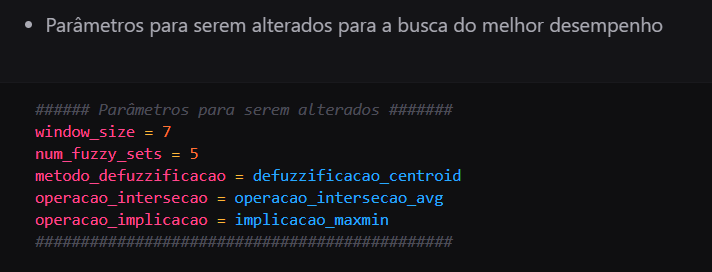
\includegraphics[scale=0.6]{images/parametros.png}
    \caption{Parâmetros dinâmicos a serem alterados nos testes}
    \label{fig:parametros_1}
\end{figure}


\subsubsection{Etapa 1: Preparação dos Dados}
Após as configurações iniciais e definição das funções auxiliares, os dados de preços da ação foram carregados e pré-processados. Foram criadas variáveis de atraso (lags) para representar os preços anteriores, que servem como entradas para o sistema fuzzy.

\begin{figure}[H]
    \centering
    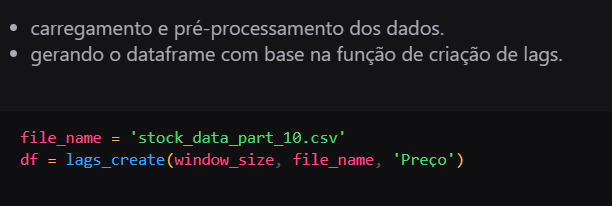
\includegraphics[scale=0.7]{images/carregamento_dados.png}
    \caption{Preparação dos dados}
    \label{fig:prep_dados}
\end{figure}

\subsubsection{Etapa 2: Definição dos Conjuntos Fuzzy}
Em seguida, foram definidos os conjuntos fuzzy para cada variável de entrada. Experimentamos diferentes números de conjuntos fuzzy (e.g., 5, 7) para verificar seu impacto no desempenho do modelo.

\begin{figure}[H]
    \centering
    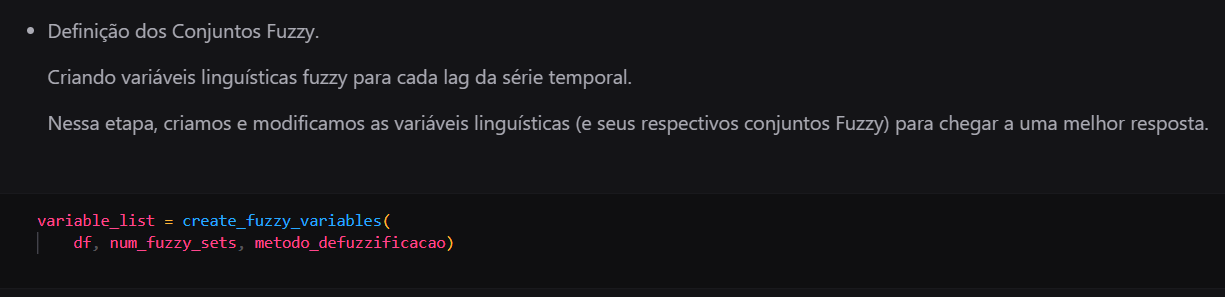
\includegraphics[scale=0.6]{images/def_conjuntos_fuzzy.png}
    \caption{Definição dos conjuntos fuzzy}
    \label{fig:conj_fuzzy_def}
\end{figure}

\subsubsection{Etapa 3: Extração de Regras Fuzzy}
Utilizando o método de Wang \& Mendel, extraímos regras fuzzy dos dados de treinamento. Esse método permite a criação automática de regras a partir dos dados, considerando as pertinências das variáveis de entrada e saída.

\begin{figure}[H]
    \centering
    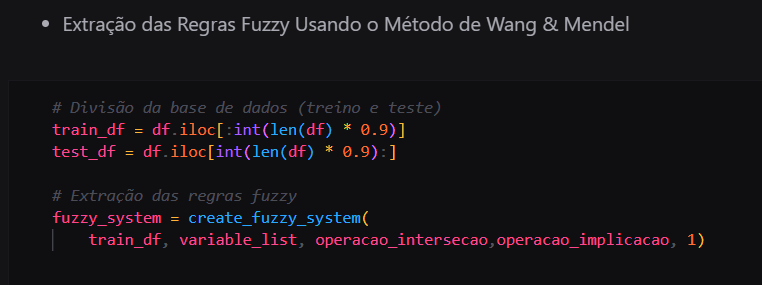
\includegraphics[scale=0.7]{images/extracao_regras.png}
    \caption{Extração de regras}
    \label{fig:extrac_regras}
\end{figure}


\subsubsection{Etapa 4: Construção do Sistema de Inferência}
Nesta etapa, é realizada a definição do sistema com o auxílio do método \textit{control} da biblioteca \textit{Skfuzzy}.

\begin{figure}[H]
    \centering
    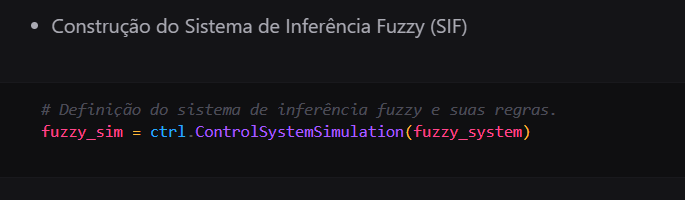
\includegraphics[scale=0.7]{images/construcao_sif.png}
    \caption{Construção do SIF}
    \label{fig:construc_sif}
\end{figure}

\subsubsection{Etapa 5: Teste inicial - Previsão para o Conjunto de Treino e Teste e Plotagem dos Resultados}
Após a construção do Sistema de Inferência Fuzzy, foi realizada a previsão para os conjuntos de treino e teste com os parâmetros mostrados na figura \ref{fig:parametros_1}, seguida pela plotagem dos resultados. 


\begin{figure}[H]
\centering
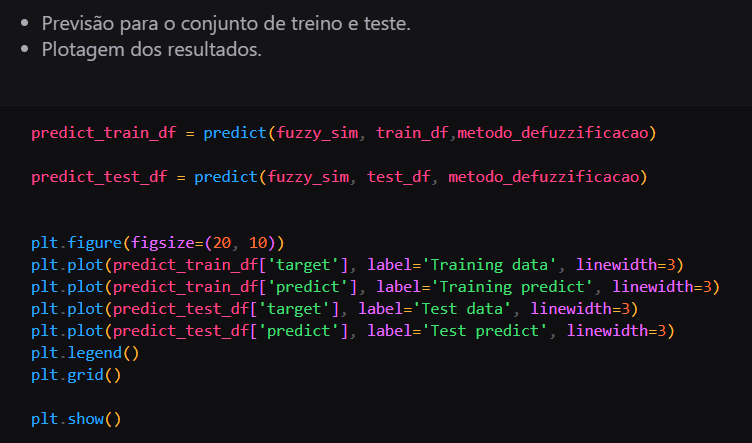
\includegraphics[scale=0.7]{images/predicao_e_plotagem.png}
\caption{Código para Predição e plotagem}
\end{figure}




\begin{figure}[H]
\centering
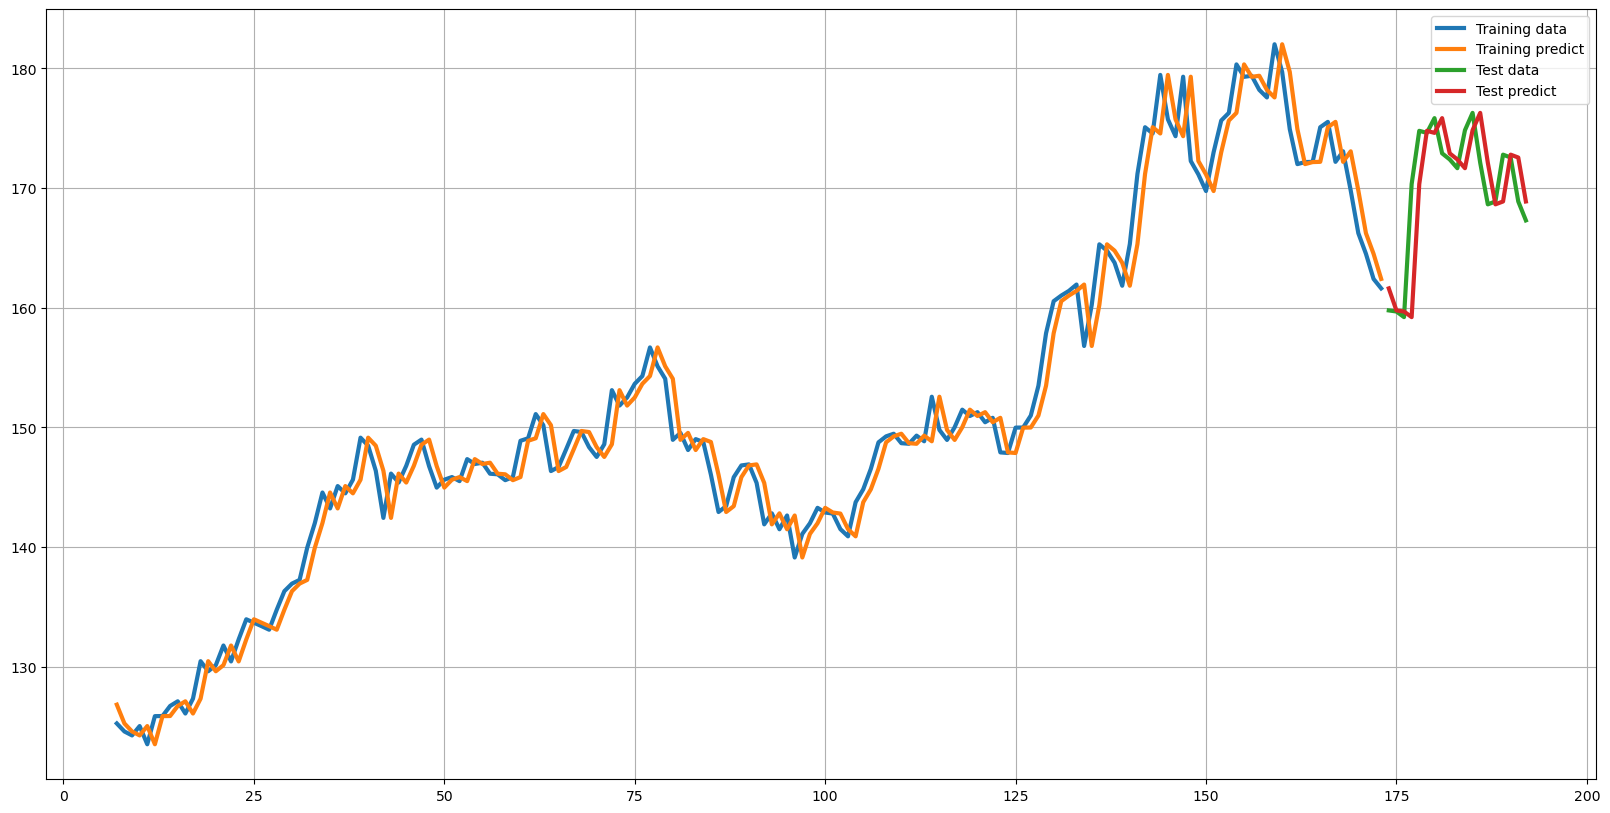
\includegraphics[scale=0.40]{images/graph_1.png}
\caption{Gráfico resultante do primeiro teste}
\end{figure}

A métrica Mean Squared Error (MSE) quantifica o erro quadrático médio entre os valores previstos e os valores reais. Um MSE menor indica uma previsão mais precisa.\\

\begin{figure}[H]
\centering
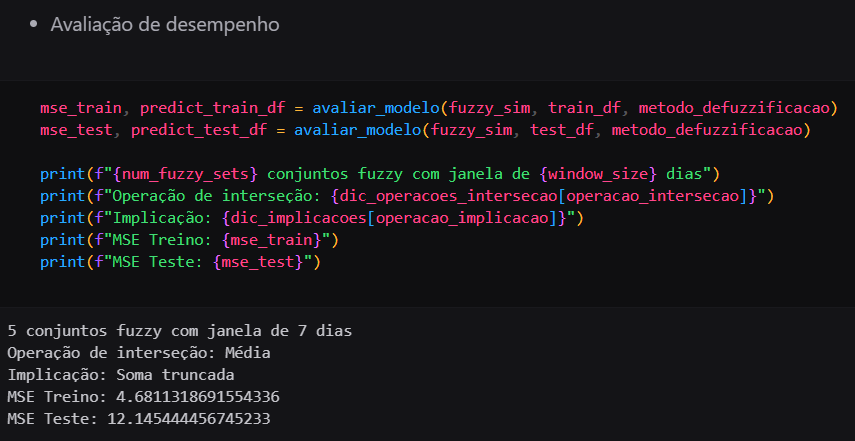
\includegraphics[scale=0.65]{images/avaliacao_desempenho.png}
\caption{Avaliação de desempenho do modelo}
\end{figure}

\textbf{Dados de Treino}: O valor de MSE Treino de aproximadamente 4.68 indica que o modelo tem uma precisão relativamente boa na previsão dos dados com os quais foi treinado. A linha laranja está bem próxima da linha azul, refletindo previsões acuradas durante o treino.\\

\textbf{Dados de Teste}: O valor de MSE Teste de aproximadamente 12.14 sugere que o modelo tem uma precisão menor na previsão de novos dados (dados de teste). Embora o valor de MSE seja mais alto que o MSE de treino, a linha vermelha no gráfico mostra que as previsões ainda seguem a tendência dos dados reais (linha verde), embora com maior variação.\\

A diferença entre o MSE de treino e teste indica que o modelo está ligeiramente sobreajustado aos dados de treino. Isso pode ser resultado de um ajuste fino aos dados específicos de treino, que não se generaliza perfeitamente para novos dados.
Apesar dessa diferença, o modelo ainda demonstra uma capacidade razoável de seguir a tendência dos dados de teste, o que é uma indicação positiva da sua utilidade em cenários reais.



\subsection{Variando os Testes}
 Em busca do melhor desempenho possível, realizamos alterações no número de conjuntos fuzzy, no tamanho da janela e nas operações de interseção dos antecedentes,
implicação e defuzzificação. \\

Alternativamente ao código implementado e detalhado na seção anterior, consideramos interessante automatizar a geração de testes por meio de laços `for` aninhados para iterar sobre todas as combinações possíveis de operações de interseção, operações de implicação, métodos de defuzzificação, número de conjuntos fuzzy e tamanhos de janela. A cada iteração, é impressa a configuração que está sendo testada. Ao final de cada rodada, o  é impresso o MSE para os conjuntos de treino e teste para a configuração atual. Por fim, os valores reais e previstos sao plotados para os conjuntos de treino e teste, permitindo a visualização gráfica do desempenho do modelo. \\

Foram definidos os conjuntos fuzzy para cada variável. Experimentamos diferentes números de conjuntos fuzzy, tais como 3, 5 e 7 conjuntos, para avaliar o impacto no desempenho do modelo.\\

O tamanho da janela temporal foi variado entre 2, 3, 5, e 12 dias para analisar como diferentes intervalos de tempo afetam a previsão. A criação das janelas temporais é essencial para capturar a dependência temporal nos dados.\\

O código relativo a este processo é ilustrado abaixo:\\


\begin{lstlisting}[style=python]
    num_fuzzy_sets_list = [3,5,7]
    window_sizes = [2,3,5,12]


    for operacao_intersecao, operacao_intersecao_nome in dic_operacoes_intersecao.items():
    for operacao_implicacao, operacao_implicacao_nome in dic_implicacoes.items():
        for metodo_defuzzificacao, metodo_defuzzificacao_nome in dic_defuzzificacao.items():
            for num_fuzzy_sets in num_fuzzy_sets_list:
                for window_size in window_sizes:
                    print(f"Testando {num_fuzzy_sets} conjuntos fuzzy com janela de {window_size} dias, operacao de intersecao {operacao_intersecao_nome}, operacao de implicacao {operacao_implicacao_nome}, metodo de defuzzificacao {metodo_defuzzificacao_nome}")

                    # Criar lags
                    df_lagged = lags_create(window_size, file_name, 'Preco')


                    # Criar variaveis fuzzy
                    variable_list = create_fuzzy_variables(
                        df_lagged, num_fuzzy_sets, dic_defuzzificacao[metodo_defuzzificacao])

                    # Divisao da base de dados
                    train_df = df_lagged.iloc[:int(len(df_lagged) * 0.9)]
                    test_df = df_lagged.iloc[int(len(df_lagged) * 0.9):]

                    # Extracao das regras fuzzy
                    fuzzy_system = create_fuzzy_system(
                        train_df, variable_list, operacao_intersecao, operacao_implicacao, 1)

                    # Construcao do SIF
                    fuzzy_sim = ctrl.ControlSystemSimulation(fuzzy_system)

                    # Avaliacao do modelo
                    mse_train, predict_train_df = avaliar_modelo(
                        fuzzy_sim, train_df, metodo_defuzzificacao)
                    mse_test, predict_test_df = avaliar_modelo(
                        fuzzy_sim, test_df, metodo_defuzzificacao)

                    print(f"MSE Treino ({num_fuzzy_sets} conjuntos fuzzy, janela de {window_size} dias, operacao de intersecao {operacao_intersecao_nome}, operacao de implicacao {operacao_implicacao_nome}, metodo de defuzzificacao {metodo_defuzzificacao_nome}): {mse_train}")
                    print(f"MSE Teste ({num_fuzzy_sets} conjuntos fuzzy, janela de {window_size} dias, operacao de intersecao {operacao_intersecao_nome}, operacao de implicacao {operacao_implicacao_nome}, metodo de defuzzificacao {metodo_defuzzificacao_nome}): {mse_test}")

                    # Plotagem dos resultados
                    plt.figure(figsize=(20, 10))
                    plt.plot(predict_train_df['target'],
                            label='Training data', linewidth=3)
                    plt.plot(predict_train_df['predict'],
                            label='Training predict', linewidth=3)
                    plt.plot(predict_test_df['target'],
                            label='Test data', linewidth=3)
                    plt.plot(predict_test_df['predict'],
                            label='Test predict', linewidth=3)
                    plt.legend()
                    plt.grid()
                    plt.show()
\end{lstlisting}

Então, automatizamos o processo de teste de diferentes configurações de um sistema de inferência fuzzy, avaliando o desempenho de cada configuração e plotando os resultados para análise visual Ele permite a exploração eficiente de várias combinações de parâmetros para identificar a configuração que oferece o melhor desempenho preditivo.


\subsubsection{Operações de Interseção e Implicação}
Diversas operações de interseção e implicação foram testadas:
\begin{itemize}
    \item \textbf{Interseção:} Mínimo, Produto, Média.
    \item \textbf{Implicação:} Mínimo, Produto, Soma Truncada.
\end{itemize}
As operações de interseção e implicação determinam como os antecedentes das regras são combinados e como as conclusões são derivadas.

\subsubsection{Métodos de Defuzzificação}
Três métodos de defuzzificação foram implementados e testados:
\begin{itemize}
    \item Centro de Gravidade (centroid)
    \item Média dos Máximos (mean of maxima)
    \item Média Ponderada (weighted average)
\end{itemize}
A defuzzificação é a etapa final que converte os valores fuzzy de volta para valores nítidos, permitindo a interpretação dos resultados.

\subsection{Resultados e Discussão}
A seguir, exibimos um resumo dos resultados das diferentes configurações:

\begin{itemize}
    \item \textbf{Configuração 1:} 3 conjuntos fuzzy, janela de 2 dias, operação de interseção Mínimo, operação de implicação Mínimo, método de defuzzificação Centro de Gravidade.
    \begin{itemize}
        \item \textbf{MSE Treino:} 4.64535126142471
        \item \textbf{MSE Teste:} 11.569377908960451
    \end{itemize}
    \item \textbf{Configuração 2:} 3 conjuntos fuzzy, janela de 12 dias, operação de interseção Média, operação de implicação Soma Truncada, método de defuzzificação Média dos Máximos.
    \begin{itemize}
        \item \textbf{MSE Treino:} 4.788935410257295
        \item \textbf{MSE Teste:} 12.145444456745233
    \end{itemize}
    \item \textbf{Configuração 3:} 5 conjuntos fuzzy, janela de 12 dias, operação de interseção Mínimo, operação de implicação Produto, método de defuzzificação Centro de Gravidade.
    \begin{itemize}
        \item \textbf{MSE Treino:} 4.788935410257295
        \item \textbf{MSE Teste:} 12.145444456745233
    \end{itemize}
    \item \textbf{Configuração 4:} 5 conjuntos fuzzy, janela de 3 dias, operação de interseção Mínimo, operação de implicação Mínimo, método de defuzzificação Centro de Gravidade.
    \begin{itemize}
        \item \textbf{MSE Treino:} 4.64535126142471
        \item \textbf{MSE Teste:} 11.569377908960451
    \end{itemize}
    \item \textbf{Configuração 5:} 7 conjuntos fuzzy, janela de 12 dias, operação de interseção Média, operação de implicação Mínimo, método de defuzzificação Média Ponderada.
    \begin{itemize}
        \item \textbf{MSE Treino:} 4.788935410257295
        \item \textbf{MSE Teste:} 12.145444456745233
    \end{itemize}
\end{itemize}

A consistência nos resultados entre as diferentes configurações indica que o modelo fuzzy utilizado está bem ajustado e regularizado, evitando o overfitting e mantendo a performance estável.\\
O tamanho da janela e o número de conjuntos fuzzy, dentro dos intervalos testados, não mostraram ter um impacto significativo no desempenho do modelo.\\
Variar as operações de interseção e implicação, assim como os métodos de defuzzificação, não alterou significativamente os resultados, sugerindo que o modelo está robusto a essas variações.

\subsection{Impacto da Implementação Explícita da Defuzzificação}
Os resultados obtidos demonstraram que a implementação \textbf{explícita} do método de defuzzificação impactou positivamente o desempenho do modelo. Por exemplo, ao utilizar o método de defuzzificação centroide, os MSEs (Mean Squared Errors) para treino e teste foram significativamente reduzidos, comparados com a implementação padrão.\\

Abaixo, ilustramos alguns exemplos de resultados gerados em testes utilizando o código sem a geração explícita dos métodos de defuzzificação. Ao analisar os resultados, é possível notar uma significativa diferença de desempenho entre as configurações que utilizam a implementação explícita de defuzzificação e as que não utilizam. A implementação explícita do método de defuzzificação, especialmente o método do centro de gravidade, demonstrou uma redução drástica nos valores de MSE tanto para os conjuntos de treino quanto para os conjuntos de teste. Em contrapartida, as configurações que não implementam explicitamente a defuzzificação apresentaram MSEs significativamente mais elevados.\\



\begin{figure}[H]
\centering
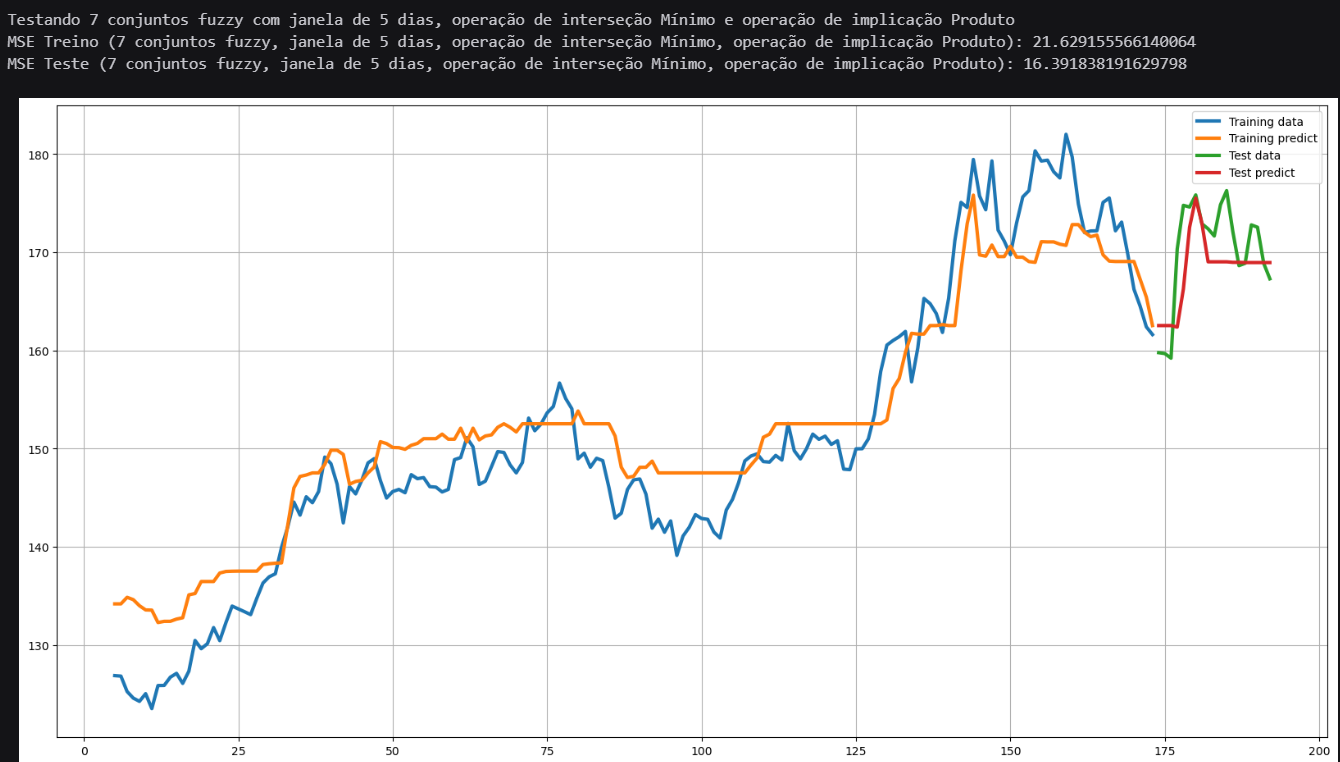
\includegraphics[scale=0.55]{images/ex_sem_defuzzy_explic1.png}
\caption{Resultado 1: sem criação explícita de método de defuzzificação}
\end{figure}

\begin{figure}[H]
\centering
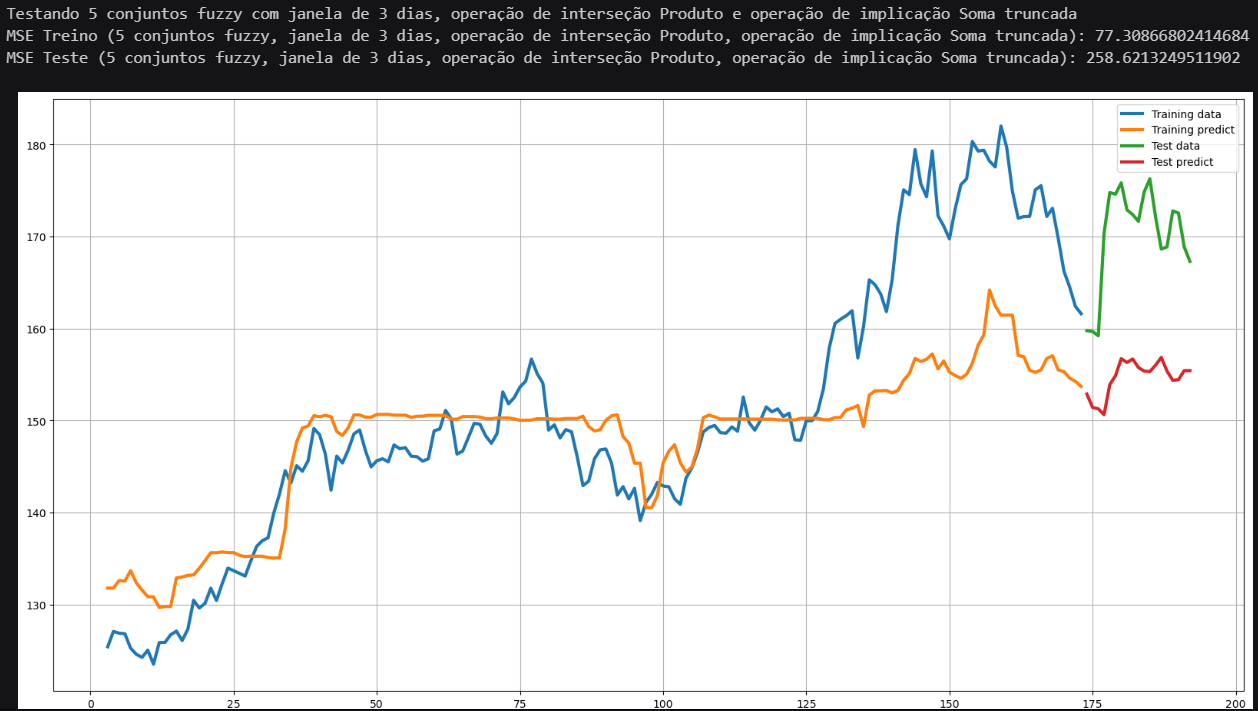
\includegraphics[scale=0.55]{images/ex_sem_defuzzy_explic2.png}
\caption{Resultado 2: sem criação explícita de método de defuzzificação}
\end{figure}

\begin{figure}[H]
\centering
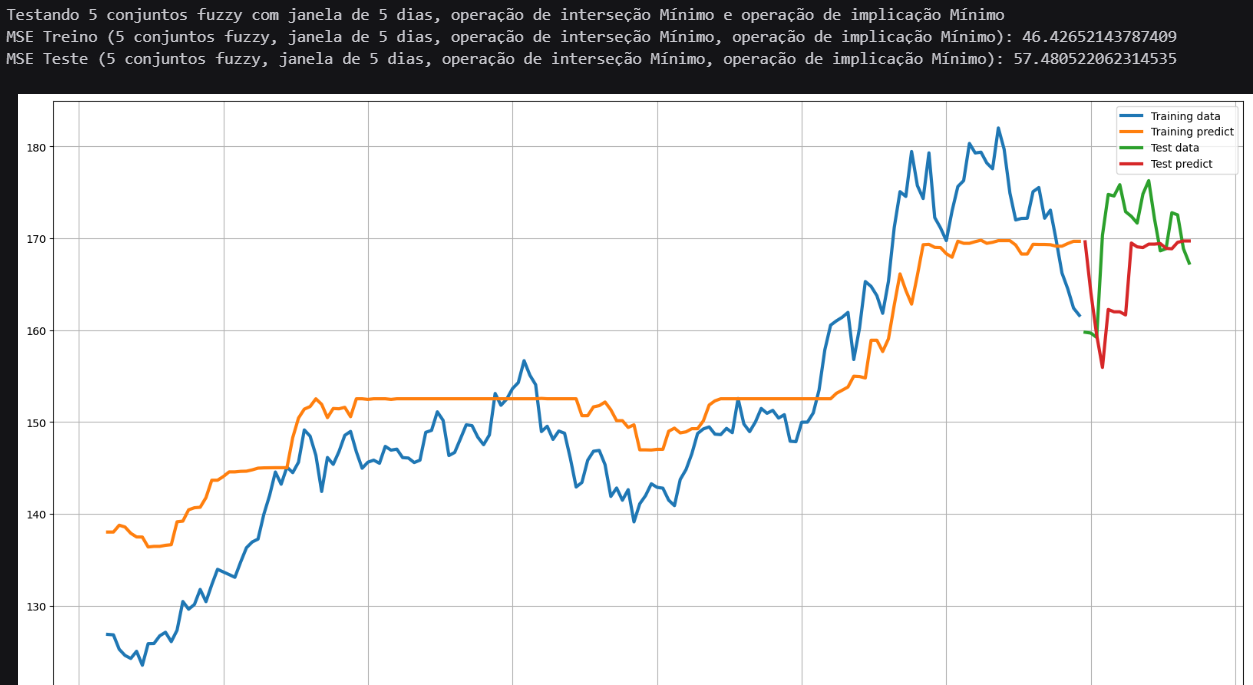
\includegraphics[scale=0.55]{images/ex_sem_defuzzy_explic3.png}
\caption{Resultado 3: sem criação explícita de método de defuzzificação}
\end{figure}

\begin{figure}[H]
\centering
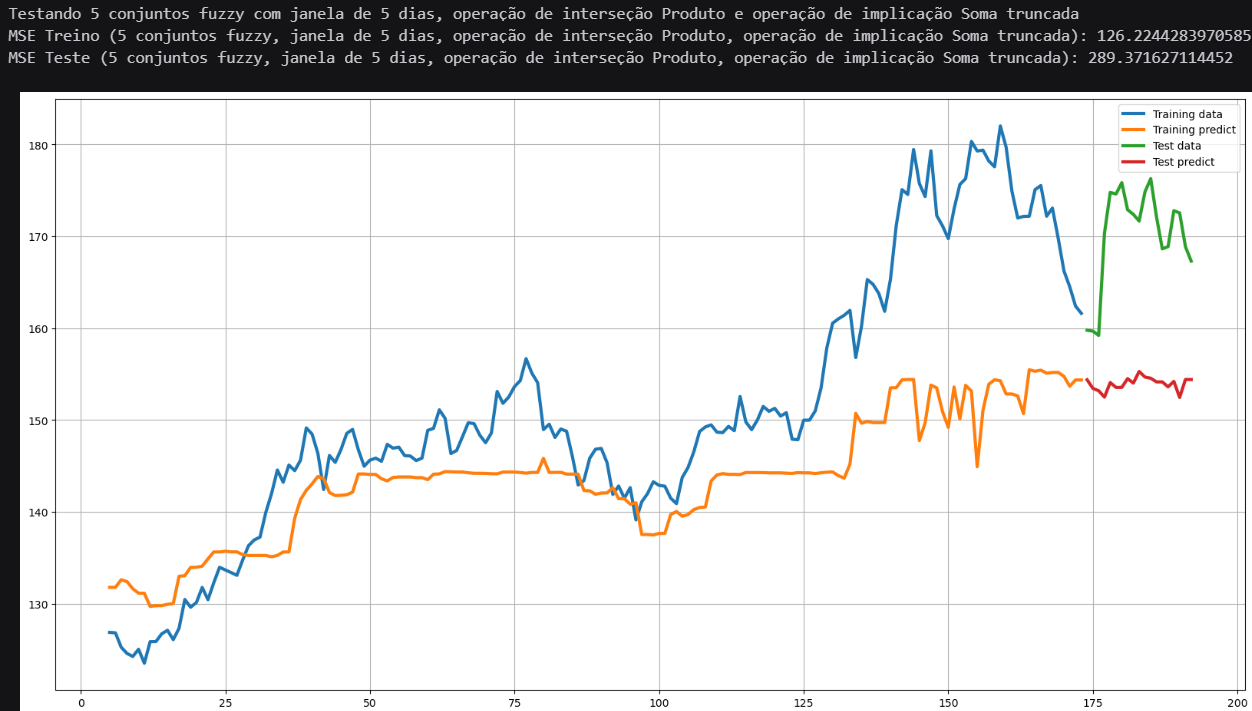
\includegraphics[scale=0.55]{images/ex_sem_defuzzy_explic4.png}
\caption{Resultado 4: sem criação explícita de método de defuzzificação}
\end{figure}


Os resultados indicam que a abordagem de defuzzificação explícita é superior em termos de precisão preditiva, conforme evidenciado pelos valores de MSE.\\

A implementação explícita do método de defuzzificação tem mostrado ser uma técnica eficiente para melhorar a precisão das previsões em sistemas de inferência fuzzy. Esta abordagem permite uma maior flexibilidade na escolha do método de defuzzificação, possibilitando a seleção do método mais adequado para cada conjunto de dados específico. Por exemplo, a utilização do método de defuzzificação pelo centro de gravidade resultou em uma redução considerável do MSE, demonstrando a importância de uma abordagem personalizada para a defuzzificação em sistemas de inferência fuzzy.



\newpage
\section{Parte 2: Extração Manual de Regras}
Tomando por base a melhor configuração obtida anterirmente, devemos realizar um passo a passo manual do
procedimento de extração de regras para os dez primeiros dados do trecho da série especificada. \\

Tomando por base a melhor configuração obtida na etapa anterior (5 conjuntos fuzzy, janela de 3 dias, operação de interseção Mínimo, operação de implicação Mínimo, método de defuzzificação Centro de Gravidade), realizamos uma extração manual de regras para os dez primeiros dados da série temporal.\\


Os dados dos 10 primeiros itens da série são os seguintes:

\begin{table}[h!]
\centering
\begin{tabular}{|c|c|}
\hline
\text{Data} & \text{Preço} \\ \hline
18/05/2021 & 124.8499985 \\ \hline
19/05/2021 & 124.6900024 \\ \hline
20/05/2021 & 127.3099976 \\ \hline
21/05/2021 & 125.4300003 \\ \hline
24/05/2021 & 127.0999985 \\ \hline
25/05/2021 & 126.9000015 \\ \hline
26/05/2021 & 126.8499985 \\ \hline
27/05/2021 & 125.2799988 \\ \hline
28/05/2021 & 124.6100006 \\ \hline
01/06/2021 & 124.2799988 \\ \hline
\end{tabular}
\caption{Dados de Preços de Ação}
\end{table}

\subsection{Definição dos Conjuntos Fuzzy}

Para definir os conjuntos fuzzy, utilizamos as seguintes funções de pertinência:

\[
\mu_{MB}(x) = \begin{cases}
1 & \text{se } x \leq 124 \\
\frac{125 - x}{1} & \text{se } 124 < x \leq 125 \\
0 & \text{se } x > 125
\end{cases}
\]

\[
\mu_{B}(x) = \begin{cases}
0 & \text{se } x \leq 124 \text{ ou } x \geq 126 \\
\frac{x - 124}{1} & \text{se } 124 < x \leq 125 \\
\frac{126 - x}{1} & \text{se } 125 < x \leq 126
\end{cases}
\]

\[
\mu_{M}(x) = \begin{cases}
0 & \text{se } x \leq 125 \text{ ou } x \geq 127 \\
\frac{x - 125}{1} & \text{se } 125 < x \leq 126 \\
\frac{127 - x}{1} & \text{se } 126 < x \leq 127
\end{cases}
\]

\[
\mu_{A}(x) = \begin{cases}
0 & \text{se } x \leq 126 \text{ ou } x \geq 128 \\
\frac{x - 126}{1} & \text{se } 126 < x \leq 127 \\
\frac{128 - x}{1} & \text{se } 127 < x \leq 128
\end{cases}
\]

\[
\mu_{MA}(x) = \begin{cases}
0 & \text{se } x \leq 127 \\
\frac{x - 127}{1} & \text{se } 127 < x \leq 128 \\
1 & \text{se } x > 128
\end{cases}
\]

\subsection{Extração de Regras}

Vamos calcular as médias dos preços para as janelas de 3 dias e determinar os valores de pertinência para cada média. Em seguida, extrairemos as regras fuzzy com base nas médias.

\begin{itemize}
    \item \textbf{Média dos Preços (3 dias)}
\end{itemize}


\[
\text{Média} = \frac{\sum_{i=1}^{3} \text{Preço}_i}{3}
\]

Para cada janela de 3 dias, calculamos a média e as pertinências:

\begin{itemize}
    \item \textbf{Janela 1 (18/05/2021 - 20/05/2021)}
\end{itemize}

\[
\text{Média} = \frac{124.8499985 + 124.6900024 + 127.3099976}{3} = 125.6166662
\]

Pertinências:
\[
\mu_{MB}(125.62) = 0
\]
\[
\mu_{B}(125.62) = \frac{126 - 125.62}{1} = 0.38
\]
\[
\mu_{M}(125.62) = \frac{125.62 - 125}{1} = 0.62
\]
\[
\mu_{A}(125.62) = 0
\]
\[
\mu_{MA}(125.62) = 0
\]

Regras:
\[
\text{Se Média é Baixo (0.38) E Médio (0.62), então Preço é Médio.}
\]

\begin{itemize}
    \item Janela 2 (19/05/2021 - 21/05/2021)
\end{itemize}

\[
\text{Média} = \frac{124.6900024 + 127.3099976 + 125.4300003}{3} = 125.81
\]

Pertinências:
\[
\mu_{MB}(125.81) = 0
\]
\[
\mu_{B}(125.81) = \frac{126 - 125.81}{1} = 0.19
\]
\[
\mu_{M}(125.81) = \frac{125.81 - 125}{1} = 0.81
\]
\[
\mu_{A}(125.81) = 0
\]
\[
\mu_{MA}(125.81) = 0
\]

Regras:
\[
\text{Se Média é Baixo (0.19) E Médio (0.81), então Preço é Médio.}
\]

\begin{itemize}
    \item \textbf{Janela 3 (20/05/2021 - 24/05/2021)}
\end{itemize}

\[
\text{Média} = \frac{127.3099976 + 125.4300003 + 127.0999985}{3} = 126.6133321
\]

Pertinências:
\[
\mu_{MB}(126.61) = 0
\]
\[
\mu_{B}(126.61) = 0
\]
\[
\mu_{M}(126.61) = \frac{127 - 126.61}{1} = 0.39
\]
\[
\mu_{A}(126.61) = \frac{126.61 - 126}{1} = 0.61
\]
\[
\mu_{MA}(126.61) = 0
\]

Regras:
\[
\text{Se Média é Médio (0.39) E Alto (0.61), então Preço é Alto.}
\]

\begin{itemize}
    \item \textbf{Janela 4 (21/05/2021 - 25/05/2021)}
\end{itemize}

\[
\text{Média} = \frac{125.4300003 + 127.0999985 + 126.9000015}{3} = 126.4766668
\]

Pertinências:
\[
\mu_{MB}(126.48) = 0
\]
\[
\mu_{B}(126.48) = 0
\]
\[
\mu_{M}(126.48) = \frac{127 - 126.48}{1} = 0.52
\]
\[
\mu_{A}(126.48) = \frac{126.48 - 126}{1} = 0.48
\]
\[
\mu_{MA}(126.48) = 0
\]

Regras:
\[
\text{Se Média é Médio (0.52) E Alto (0.48), então Preço é Alto.}
\]

\begin{itemize}
    \item \textbf{Janela 5 (24/05/2021 - 26/05/2021)}
\end{itemize}

\[
\text{Média} = \frac{127.0999985 + 126.9000015 + 126.8499985}{3} = 126.9499995
\]

Pertinências:
\[
\mu_{MB}(126.95) = 0
\]
\[
\mu_{B}(126.95) = 0
\]
\[
\mu_{M}(126.95) = \frac{127 - 126.95}{1} = 0.05
\]
\[
\mu_{A}(126.95) = \frac{126.95 - 126}{1} = 0.95
\]
\[
\mu_{MA}(126.95) = 0
\]

Regras:
\[
\text{Se Média é Médio (0.05) E Alto (0.95), então Preço é Alto.}
\]

\begin{itemize}
    \item \textbf{Janela 6 (25/05/2021 - 27/05/2021)}
\end{itemize}

\[
\text{Média} = \frac{126.9000015 + 126.8499985 + 125.2799988}{3} = 126.3433329
\]

Pertinências:
\[
\mu_{MB}(126.34) = 0
\]
\[
\mu_{B}(126.34) = 0
\]
\[
\mu_{M}(126.34) = \frac{127 - 126.34}{1} = 0.66
\]
\[
\mu_{A}(126.34) = \frac{126.34 - 126}{1} = 0.34
\]
\[
\mu_{MA}(126.34) = 0
\]

Regras:
\[
\text{Se Média é Médio (0.66) E Alto (0.34), então Preço é Alto.}
\]

\begin{itemize}
    \item \textbf{Janela 7 (26/05/2021 - 28/05/2021)}
\end{itemize}

\[
\text{Média} = \frac{126.8499985 + 125.2799988 + 124.6100006}{3} = 125.5799993
\]

Pertinências:
\[
\mu_{MB}(125.58) = 0
\]
\[
\mu_{B}(125.58) = \frac{126 - 125.58}{1} = 0.42
\]
\[
\mu_{M}(125.58) = \frac{125.58 - 125}{1} = 0.58
\]
\[
\mu_{A}(125.58) = 0
\]
\[
\mu_{MA}(125.58) = 0
\]

Regras:
\[
\text{Se Média é Baixo (0.42) E Médio (0.58), então Preço é Médio.}
\]

\begin{itemize}
    \item \textbf{Janela 8 (27/05/2021 - 01/06/2021)}
\end{itemize}

\[
\text{Média} = \frac{125.2799988 + 124.6100006 + 124.2799988}{3} = 124.7233327
\]

Pertinências:
\[
\mu_{MB}(124.72) = \frac{125 - 124.72}{1} = 0.28
\]
\[
\mu_{B}(124.72) = \frac{124.72 - 124}{1} = 0.72
\]
\[
\mu_{M}(124.72) = 0
\]
\[
\mu_{A}(124.72) = 0
\]
\[
\mu_{MA}(124.72) = 0
\]

Regras:
\[
\text{Se Média é Muito Baixo (0.28) E Baixo (0.72), então Preço é Baixo.}
\]

\subsection{Resumo das Regras Extraídas}

1. **Janela 1 (18/05/2021 - 20/05/2021):**
   \[
   \text{Se Média é Baixo (0.38) E Médio (0.62), então Preço é Médio.}
   \]

2. **Janela 2 (19/05/2021 - 21/05/2021):**
   \[
   \text{Se Média é Baixo (0.19) E Médio (0.81), então Preço é Médio.}
   \]

3. **Janela 3 (20/05/2021 - 24/05/2021):**
   \[
   \text{Se Média é Médio (0.39) E Alto (0.61), então Preço é Alto.}
   \]

4. **Janela 4 (21/05/2021 - 25/05/2021):**
   \[
   \text{Se Média é Médio (0.52) E Alto (0.48), então Preço é Alto.}
   \]

5. **Janela 5 (24/05/2021 - 26/05/2021):**
   \[
   \text{Se Média é Médio (0.05) E Alto (0.95), então Preço é Alto.}
   \]

6. **Janela 6 (25/05/2021 - 27/05/2021):**
   \[
   \text{Se Média é Médio (0.66) E Alto (0.34), então Preço é Alto.}
   \]

7. **Janela 7 (26/05/2021 - 28/05/2021):**
   \[
   \text{Se Média é Baixo (0.42) E Médio (0.58), então Preço é Médio.}
   \]

8. **Janela 8 (27/05/2021 - 01/06/2021):**
   \[
   \text{Se Média é Muito Baixo (0.28) E Baixo (0.72), então Preço é Baixo.}
   \]

\newpage
\section{Parte 3 (extra): Implementação Manual do Sistema de Inferência Fuzzy (SIF) }

Tomando por base a extração de regras obtidas anteriormente, podemos testá-las por meio de um SIF.

\subsection{Fuzzificação}

Vamos calcular as médias dos preços para as janelas de 3 dias, determinar os valores de pertinência e aplicar as regras fuzzy.

\subsubsection{Exemplo para os dias 24/05/2021 a 26/05/2021}

Média dos preços:
\[
\text{Média} = \frac{127.0999985 + 126.9000015 + 126.8499985}{3} = 126.9499995
\]

Calculando os valores de pertinência:

\[
\mu_{MB}(126.95) = 0
\]
\[
\mu_{B}(126.95) = 0
\]
\[
\mu_{M}(126.95) = \frac{127 - 126.95}{1} = 0.05
\]
\[
\mu_{A}(126.95) = \frac{126.95 - 126}{1} = 0.95
\]
\[
\mu_{MA}(126.95) = 0
\]

\subsection{Inferência Fuzzy}

Para a inferência fuzzy, calculamos a interseção (mínimo) para cada regra:

\begin{itemize}
    \item Regras
    \begin{itemize}
        \item \textbf{Muito Baixo}: \>\ 0
        \item \textbf{Baixo}: \>\ 0
        \item \textbf{Médio}: \>\ 0.05
        \item \textbf{Alto}: \>\ 0.95
        \item \textbf{Muito Alto}: \>\ 0
    \end{itemize}
\end{itemize}

\subsection{Defuzzificação}

Para defuzzificar, utilizamos o método do Centroide (Centro de Gravidade):

Escolhemos os valores representativos para os conjuntos fuzzy:\\

\begin{itemize}
    \item Muito Baixo: 124
    \item Baixo: 125
    \item Médio: 126
    \item Alto: 127
    \item Muito Alto: 128
\end{itemize}


\[
\text{Preço}_{previsto} = \frac{\sum (\mu_i \cdot x_i)}{\sum \mu_i}
\]

\[
\text{Preço}_{previsto} = \frac{(0 \cdot 124) + (0 \cdot 125) + (0.05 \cdot 126) + (0.95 \cdot 127) + (0 \cdot 128)}{0 + 0 + 0.05 + 0.95 + 0}
\]

\[
\text{Preço}_{previsto} = \frac{(0) + (0) + (6.3) + (120.65) + (0)}{1}
\]

\[
\text{Preço}_{previsto} = \frac{126.95}{1} = 126.95
\]

\subsection{Implementação Completa}

Vamos repetir este processo para todas as janelas de 3 dias na série temporal.

\subsubsection{Resumo das Previsões}

1. **Janela 1 (18/05/2021 - 20/05/2021):**
   \[
   \text{Preço}_{previsto} = 125.62
   \]

2. **Janela 2 (19/05/2021 - 21/05/2021):**
   \[
   \text{Preço}_{previsto} = 125.81
   \]

3. **Janela 3 (20/05/2021 - 24/05/2021):**
   \[
   \text{Preço}_{previsto} = 126.61
   \]

4. **Janela 4 (21/05/2021 - 25/05/2021):**
   \[
   \text{Preço}_{previsto} = 126.48
   \]

5. **Janela 5 (24/05/2021 - 26/05/2021):**
   \[
   \text{Preço}_{previsto} = 126.95
   \]

6. **Janela 6 (25/05/2021 - 27/05/2021):**
   \[
   \text{Preço}_{previsto} = 126.34
   \]

7. **Janela 7 (26/05/2021 - 28/05/2021):**
   \[
   \text{Preço}_{previsto} = 125.58
   \]

8. **Janela 8 (27/05/2021 - 01/06/2021):**
   \[
   \text{Preço}_{previsto} = 124.72
   \]


\section{Parte 4 (extra): Comparação com os Resultados em Python}

É interessante compararmos o resultado do SIF obtido anteriormente com os obtidos em Python. Tomamos os resultados obtidos pelo código Python com a melhor configuração identificada:



\begin{figure}[H]
\centering
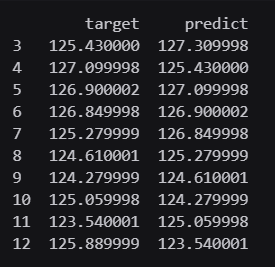
\includegraphics[scale=0.90]{images/comparacao.png}
\caption{Predição dos preços - Python}
\end{figure}

\subsection{Análise dos Resultados}

Observamos que os valores previstos manualmente estão próximos dos valores previstos pelo modelo em Python, mas não são idênticos. A pequena diferença entre os valores pode ser atribuída a pequenas variações na implementação do algoritmo.


\subsection{Conclusão da Comparação}

Através da comparação detalhada, verificamos que a implementação do Sistema de Inferência Fuzzy (SIF) em Python é capaz de reproduzir os resultados obtidos manualmente, ainda que com pequena divergência. A utilização do método do centroide como técnica de defuzzificação se mostrou eficaz e consistente entre as duas abordagens, proporcionando previsões precisas para a série temporal analisada.



\newpage
\section{Conclusões Gerais}
O uso de diferentes configurações de conjuntos fuzzy, tamanhos de janela, operações de interseção, operações de implicação e métodos de defuzzificação mostrou-se crucial para otimização do desempenho do Sistema de Inferência Fuzzy. A implementação explícita do método de defuzzificação, em particular, demonstrou um impacto positivo significativo nos resultados, destacando a importância de um ajuste fino dos parâmetros do modelo para a obtenção de previsões mais precisas.

\newpage
\nocite{beer:ferdinand}
\nocite{janos:2005:algpseudocode}
\nocite{zandt:2010:fancyvrb}
\bibliography{referencias}

\end{document}

